\begin{figure}[htbp]
\centering
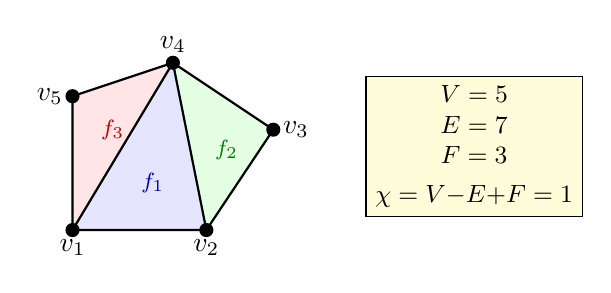
\begin{tikzpicture}[scale=0.85]
  \coordinate (v1) at (0,0);
  \coordinate (v2) at (2,0);
  \coordinate (v3) at (3,1.5);
  \coordinate (v4) at (1.5,2.5);
  \coordinate (v5) at (0,2);
  \fill[blue!10] (v1)--(v2)--(v4)--cycle;
  \fill[green!10] (v2)--(v3)--(v4)--cycle;
  \fill[red!10] (v1)--(v4)--(v5)--cycle;
  \draw[thick] (v1)--(v2) (v2)--(v3) (v3)--(v4) (v4)--(v5) (v5)--(v1);
  \draw[thick] (v1)--(v4) (v2)--(v4);
  \foreach \v/\name/\pos in {v1/$v_1$/below,v2/$v_2$/below,v3/$v_3$/right,v4/$v_4$/above,v5/$v_5$/left} {
    \fill (\v) circle (3pt) node[\pos] {\name};
  }
  \node[blue!70!black,font=\footnotesize] at (1.2,0.7) {$f_1$};
  \node[green!50!black,font=\footnotesize] at (2.3,1.2) {$f_2$};
  \node[red!70!black,font=\footnotesize] at (0.6,1.5) {$f_3$};
  \node[draw,rectangle,fill=yellow!15,font=\small,align=center] at (6,1.25) {$V=5$\\$E=7$\\$F=3$\\[3pt]$\chi = V{-}E{+}F = 1$};
\end{tikzpicture}
\caption{A triangle mesh with vertices $v_i$, edges, and faces $f_j$. The Euler characteristic $\chi = V - E + F$ is a topological invariant.}
\label{fig:mesh_connectivity}
\end{figure}
